
\subsection{Iteración 1}

Se busca diseñar las técnicas básicas que se usarán para evaluar las pruebas. En concreto encontrar las herramientas que ofrecen Unity y VRTK y cual es la mejor forma de utilizarlas para detectar que los movimientos y las acciones del jugador son las adecuadas para cada una de las pruebas.

\subsubsection{Pruebas de posición}

Hay varias pruebas que dependen exclusivamente de la posición de los mandos en el espacio virtual, por lo que es esencial poder hacer un seguimiento de su posición en todo momento. Asignando una serie de posiciones para cada controlador durante la prueba y conociendo su posición real se podría determinar si el jugador está realizando el movimiento adecuado.

Unity trabaja con un sistema de coordenadas cartesianas y todos los objetos del juego tienen un atributo que indica su posición en dicho sistema (figura \ref{fig:E2_transform}), por lo que es sencillo obtener este dato.

\begin{figure}
  \centering
    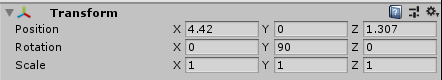
\includegraphics[width=0.9\textwidth]{04.Desarrollo/02.Entrega2/01.Iteracion2_1/00.Figuras/01.transform.png}
    \caption{Ejemplo del atributo Transform en Unity que representa la posición de un objeto en el espacio.}
    \label{fig:E2_transform}
\end{figure}

Por desgracia, no se puede basar el sistema únicamente en la posición exacta del mando, es necesario dar ciertos márgenes que ayuden al jugador a mantener el mando dentro de una zona que será tomada como válida. Una opción sería definir un punto del espacio y una distancia máxima a la que el mando se puede encontrar para considerarse una posición correcta. Unity incorpora de forma nativa un objeto llamado ‘trigger’. Un trigger (representado en la figura  \ref{fig:E2_transform}) se trata de un objeto en el espacio virtual, de cualquier forma o tamaño, que es completamente invisible al jugador y es capaz de detectar cuando otro objeto entra dentro de él. De esta forma, se puede definir un trigger en cualquier posición que reportará al sistema cuando el mando entra o sale de su perímetro.


\begin{figure}
  \centering
    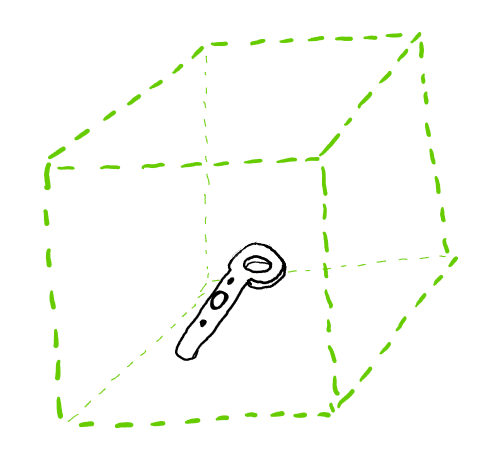
\includegraphics[width=0.5\textwidth]{04.Desarrollo/02.Entrega2/01.Iteracion2_1/00.Figuras/02.trigger.png}
    \caption{Boceto que muestra el uso de un trigger (cubo verde) para detectar el controlador en su interior.}
    \label{fig:E2_trigger}
\end{figure}


Teniendo la capacidad que ofrecen los trigger de Unity, definir las pruebas que se basan en la posición de las manos consiste en poder definir una serie de posiciones y tiempos en los que aparecerán dichos trigger para comprobar si el mando del jugador se encuentra en su interior. Puesto que los trigger son tratados como objetos comunes dentro de Unity, se pueden mover siguiendo una trayectoria y una velocidad, por lo que no solo pueden detectar posiciones, si no también evaluar el movimiento de los mandos entre dos puntos del espacio.

De esta forma ya se pueden definir algunas pruebas de movimiento:

\textbf{Posiciones.} En esta prueba se pide al jugador que adopte una pose concreta que aparece representada (figura \ref{fig:E2_poses}). Para este caso, para cada figura a imitar, es necesario definir una posición para cada mano, en dicha posición aparecerá un trigger. Si el jugador es capaz de colocar sus dos manos dentro de los trigger y mantenerlas en ellos, la prueba se dará como superada.


\begin{figure}
  \centering
    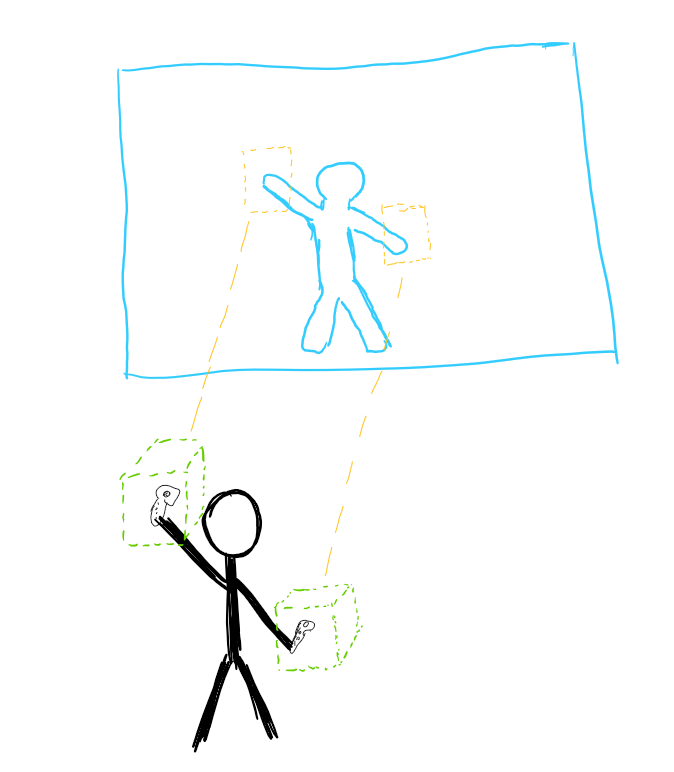
\includegraphics[width=0.5\textwidth]{04.Desarrollo/02.Entrega2/01.Iteracion2_1/00.Figuras/03.poses.png}
    \caption{Boceto que representa una posible prueba de figuras. En azul el modelo a seguir, en verde los trigger necesarios.}
    \label{fig:E2_poses}
\end{figure}

\textbf{Baile/movimientos.} (véase figura \ref{fig:E2_baile}) En este caso se puede definir un movimiento como la trayectoria que sigue un trigger dentro del espacio. Para ello es necesario definir un punto por cada momento intermedio, así como la velocidad a la que el trigger se moverá entre ellos. Si el jugador es capaz de mantener la mano dentro del espacio designado durante todo el movimiento la prueba habrá sido superada. En el caso de la prueba de baile, esta consiste en un conjunto de movimientos y posiciones uno tras otro.

\begin{figure}
  \centering
    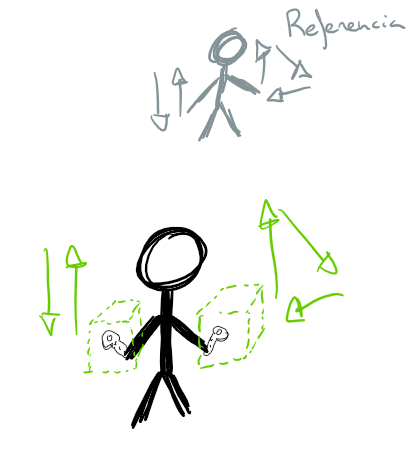
\includegraphics[width=0.5\textwidth]{04.Desarrollo/02.Entrega2/01.Iteracion2_1/00.Figuras/04.baile.png}
    \caption{Boceto representando una prueba de baile o movimientos. En gris la referencia a seguir, en verde los trigger y los movimientos que siguen.}
    \label{fig:E2_baile}
\end{figure}


\textbf{Objetivos.} Esta prueba hace que el jugador vea como varios objetos se aproximan hacia él y debe tocarlos con la mano conforme llegan a su posición, según se observa en la figura \ref{fig:E2_objetivos}. Cada objeto puede tener dos colores, el cual indica al jugador con qué mano debe tocarlo. Los objetos de color rojo se acercarán al jugador por su lado izquierdo y deberá tocarlos con su mano izquierda. Los objetos azules actuarán de la misma forma, pero para el lado derecho. Cada uno de estos objetos tendrá un ‘collider’ que es equivalente a un trigger, pero para objetos visibles al jugador, esto permitirá determinar si el jugador ha realizado la prueba de forma correcta.


\begin{figure}
  \centering
    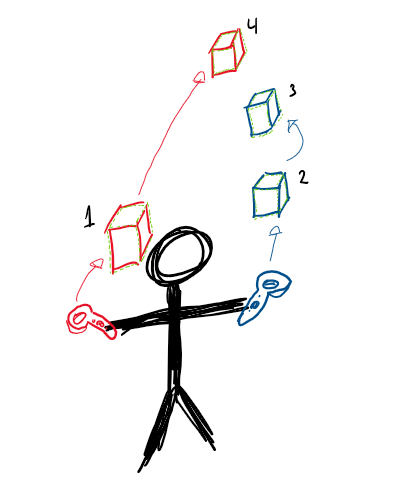
\includegraphics[width=0.5\textwidth]{04.Desarrollo/02.Entrega2/01.Iteracion2_1/00.Figuras/05.objetivos.png}
    \caption{Boceto de una prueba de objetivos. Los objetivos en azul y rojo deberán tocarse con el mando del mismo color.}
    \label{fig:E2_objetivos}
\end{figure}


\subsubsection{Pruebas de interacción}

Algunas de las pruebas requerirán que el jugador interactúe con objetos virtuales, cogiéndolos, soltándolos o de formas similares. Por suerte, estas son capacidades básicas que ofrecen SteamVR y VRTK y que ya fueron integradas en el proyecto como parte de la primera entrega. Por lo que la definición de cada prueba consistirá en gran parte de la generación de los objetos virtuales: cuáles, dónde y cómo aparecen. Así como detectar lo que el jugador hace con ellos.

Para la prueba de agrupación de objetos (véase figura \ref{fig:E2_agrupacion}) se presentarán al jugador un grupo de objetos virtuales y esté deberá descubrir su asociación y colocarlos en dos zonas separadas. Estas zonas se pueden definir usando los trigger explicados anteriormente, de modo que basta con detectar cuándo todos los objetos han sido introducidos en alguna de las dos zonas, y evaluar si cada uno está donde le corresponde.


\begin{figure}
  \centering
    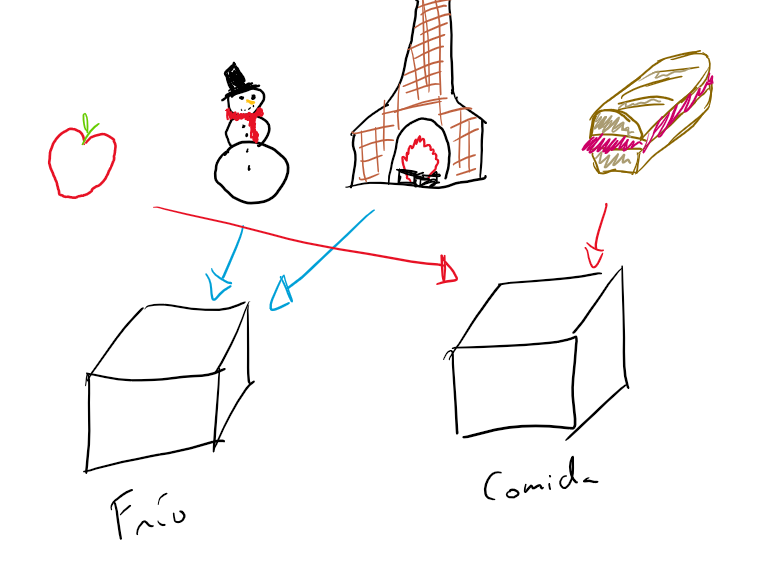
\includegraphics[width=0.5\textwidth]{04.Desarrollo/02.Entrega2/01.Iteracion2_1/00.Figuras/06.agrupacion.png}
    \caption{Boceto de la prueba de agrupación de objetos. Las categorías "frío" y "comida" no son visibles para el jugador.}
    \label{fig:E2_agrupacion}
\end{figure}

En la prueba de figuras superpuestas se mostrarán al jugador un conjunto de objetos virtuales o siluetas que se encuentran superpuestos unos con otros como se muestra en la figura \ref{fig:E2_superpuestas}. El jugador deberá averiguar de qué objetos de trata y responder seleccionando la respuesta correcta entre las disponibles que se presentarán mediante botones interactivos en RV. La funcionalidad de estos botones está proporcionada por los paquetes instalados en la entrega anterior.


\begin{figure}
  \centering
    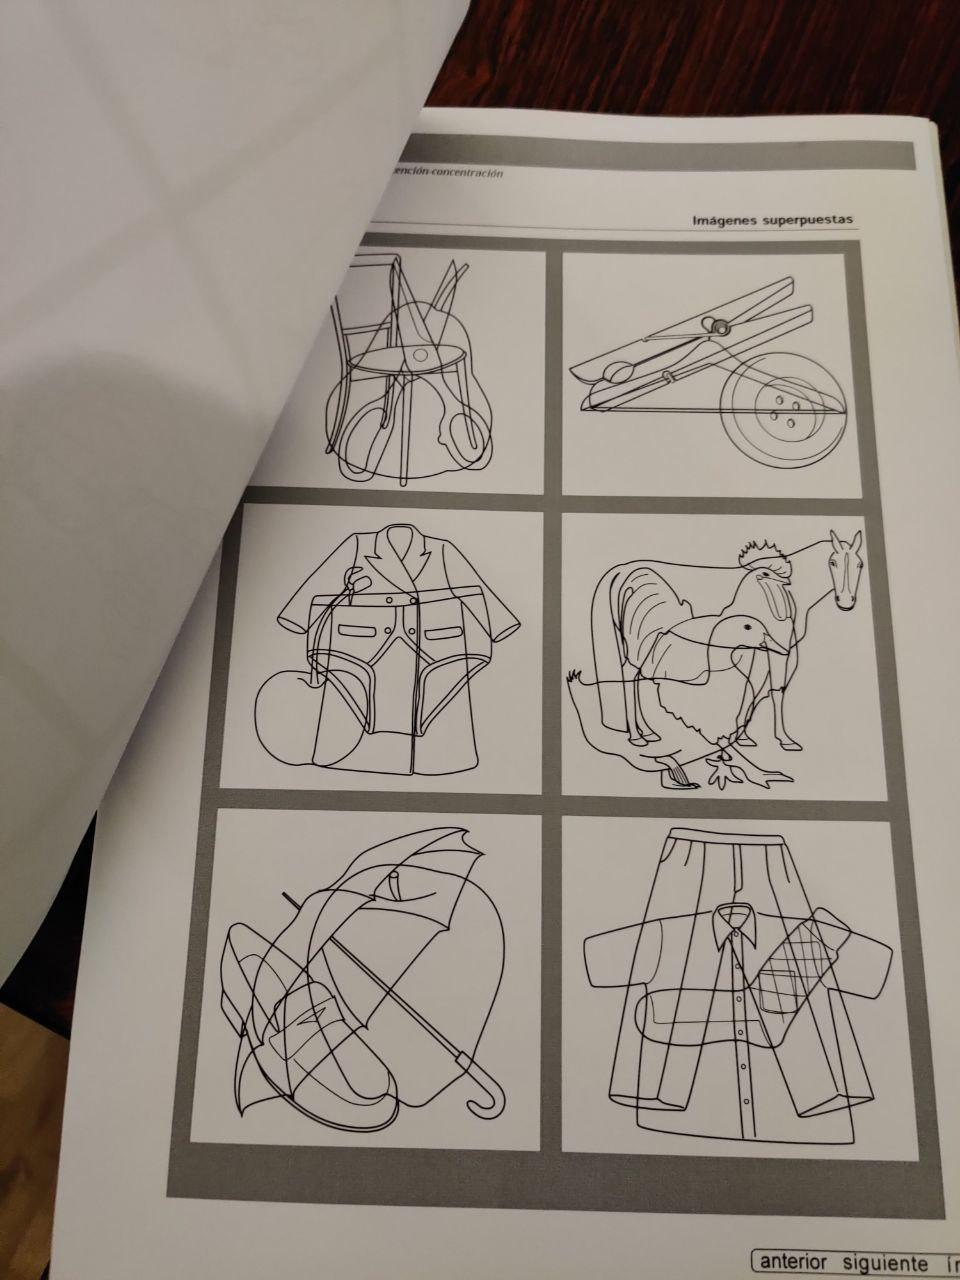
\includegraphics[width=0.5\textwidth]{04.Desarrollo/02.Entrega2/01.Iteracion2_1/00.Figuras/07.superpuestas.jpg}
    \caption{Fotografía de un ejercicio de figuras superpuestas en formato de papel.}
    \label{fig:E2_superpuestas}
\end{figure}

Para la prueba de asociación de sonidos se presentan una serie de objetos al jugador de la misma forma que en la prueba de agrupación de objetos, pero en este caso el jugador deberá escuchar un sonido y decidir qué objeto es el que produce dicho sonido, como se ilustra en la figura \ref{fig:E2_sonidos}. La única diferencia entre esta prueba y la de agrupación es que es necesario crear un objeto que sea capaz de reproducir un sonido previamente grabado y hacer que el jugador lo oiga. Por suerte esta es una funcionalidad básica de Unity.


\begin{figure}
  \centering
    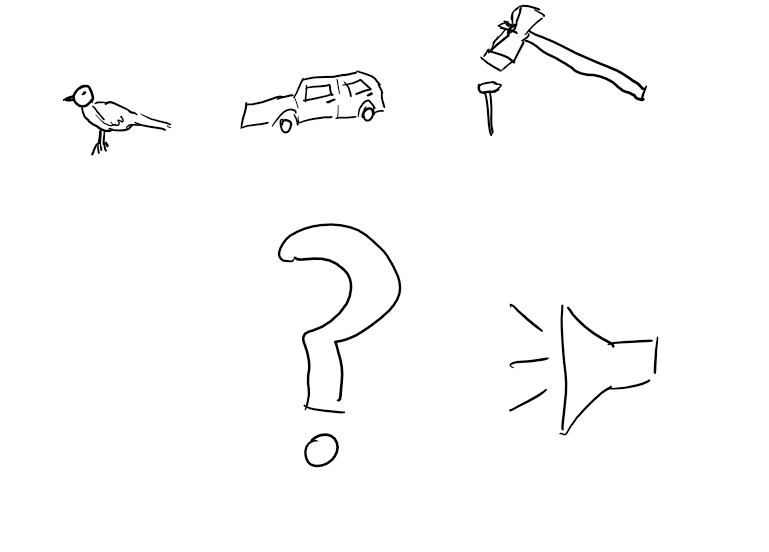
\includegraphics[width=0.5\textwidth]{04.Desarrollo/02.Entrega2/01.Iteracion2_1/00.Figuras/08.sonidos.png}
    \caption{Boceto que representa la prueba de asociación de un sonido con el objeto que lo produce.}
    \label{fig:E2_sonidos}
\end{figure}


Finalmente, para la prueba de localización de sonidos únicamente es necesario colocar un emisor de sonido en un punto del espacio rodeando al jugador. Unity es capaz de utilizar audio ambisónico, un tipo de sonido que permite al usuario localizar el punto exacto en el espacio de donde proviene dicho sonido. Por tanto, se usará esta tecnología para hacer que el jugador se gire en la dirección correcta de la que proviene el sonido. Cuando el jugador sea capaz de ver el objeto que producía el sonido, la prueba ha sido superada. 


\subsubsection{Pruebas de entorno}


Estas son las pruebas en las que no se requiere que el jugador interactúe con el entorno de manera directa. Se presenta un entorno que el jugador debe observar y escuchar. Por tanto, para la evaluación de este tipo de pruebas es necesaria la participación de una persona externa al juego, preferiblemente una persona experta en entrenamiento cognitivo que actúe de guía para el usuario. Para estas pruebas no es necesario el uso de ninguna mecánica especial salvo la generación de los objetos virtuales del entorno.

